\documentclass[11pt]{article}
\usepackage[preprint]{acl}
\usepackage{times}
\usepackage{latexsym}
\usepackage[T1]{fontenc}
\usepackage[utf8]{inputenc}
\usepackage{microtype}
\usepackage{inconsolata}
\usepackage{graphicx}
\usepackage{amsmath,amssymb}
\usepackage{booktabs,tabularx,array}
\usepackage{url}
\usepackage{placeins}
\title{Hallucination in Large Language Models:\\A Survey of Detection, Evaluation, and Mitigation}
\author{Xincheng Li \\ School of Computer Science, University of Auckland \\ Email: \texttt{xli798@aucklanduni.ac.nz}}
\newcommand{\figwide}[3]{\begin{figure*}[t]\centering\includegraphics[width=\textwidth]{figures/#1}\caption{#2}\label{#3}\end{figure*}}
\begin{document}
\maketitle
\begin{abstract}
Large language models can produce fluent assertions that are false or unsupported by their evidence. Research spans detectors, benchmarks, and interventions, but their results often concern different correctness targets. This survey organizes text-based research from 2022--2026 around error definitions, detection evidence, and useful mitigation. We distinguish world factuality from source faithfulness, compare external-evidence, sampling-based, and internal-signal detectors, and connect evaluation to training, retrieval, decoding, and revision. Factual precision alone cannot establish progress: verifier dependence, selective answering, evidence quality, and distribution shift change the interpretation of gains. We develop a comparative framework pairing correctness with information coverage, independent verification, and cost, and propose tests of generalization and reliability. The companion literature collection and supporting materials are available at \url{https://github.com/lixincheng-xcl/LLM-Hallucination-Survey}.
\end{abstract}
\begin{figure}[t]
\centering
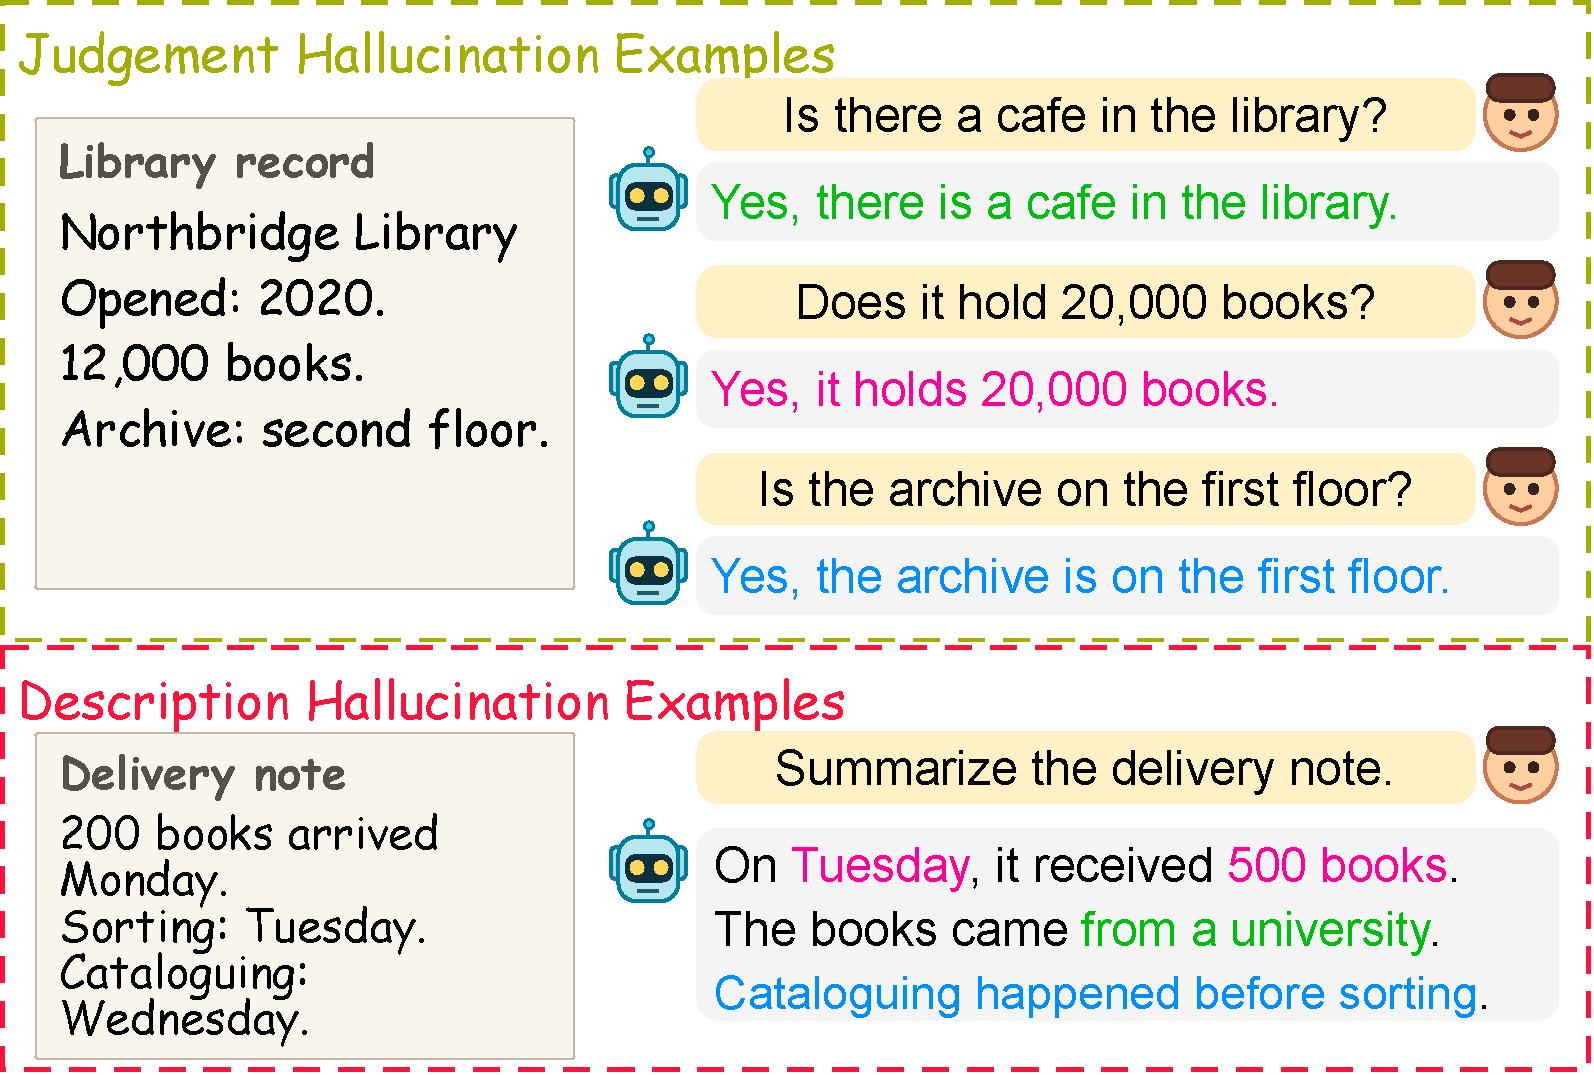
\includegraphics[width=\columnwidth]{figures/Fig1_hallucination_examples.pdf}
\caption{Hallucination examples in source-grounded question answering and summarization. Green marks unsupported additions, pink attribute errors, and blue relation errors. The cafe claim is unsupported by the record; this does not establish world falsity. See page~\pageref{app:example-large} for an enlarged view.}
\label{fig:examples}
\end{figure}
\section{Introduction}
A fluent answer from a large language model (LLM) is not necessarily justified. In question answering (QA), a model may repeat a misconception; in summarization, it may add a plausible detail absent from the source. Both are called hallucinations, although their correctness criteria differ: source-unsupported content can be factually correct \citep{lin-etal-2022-truthfulqa,cao-etal-2022-hallucinated}. Collapsing these settings obscures what a system improves.


In Figure~\ref{fig:examples}, the library record supports 12,000 books and a second-floor archive. The cafe assertion lacks support; the changed count and location contradict the record. The delivery summary also invents a university source and reverses events. Verification must specify the claim and its reference evidence.

Building on the broad factuality review of \citet{wang-etal-2024-factuality}, we connect each method's evidence and access assumptions to the evaluation target it can support. This comparison distinguishes better correction from gains caused by withholding information or changing the verifier. Three questions organize the synthesis: \textbf{RQ1}, what reference frame defines an error; \textbf{RQ2}, what evidence and access enable detection; and \textbf{RQ3}, when does mitigation improve useful generation?

\figwide{Fig2_survey_structure.pdf}{The structure of this survey. Green boxes list representative studies for each branch.}{fig:structure}
\paragraph{Scope and organization.}
This narrative survey covers 2022--2026 ACL-family research on text-based QA, long-form generation, summarization, dialogue, and retrieval-augmented generation (RAG), supplemented by mechanism-defining studies from other venues. Figure~\ref{fig:structure} maps concepts (\S\ref{sec:background}), detection (\S\ref{sec:detection}), evaluation (\S\ref{sec:evaluation}), mitigation (\S\ref{sec:mitigation}), and analysis (\S\ref{sec:analysis}). Appendix~\ref{app:selection} gives the selection criteria. Multimodal perception and general reasoning are outside the scope.

\section{Concepts and Scope}\label{sec:background}
\figwide{Fig2_survey_structure.pdf}{The structure of this survey. Green leaves locate representative studies. Branches navigate detection signals, evaluation targets, and interventions, rather than define mutually exclusive classes. Tree design adapted from \citet{liu-etal-2025-logical-design}; content is specific to this survey.}{fig:structure}
\subsection{Reference frames}
\emph{World factuality} concerns agreement with externally established facts; \emph{source faithfulness} concerns support by supplied evidence. Neither entails the other: a response can repeat a false source faithfully or add a true but unlicensed detail \citep{cao-etal-2022-hallucinated,adlakha-etal-2024-evaluating}. BEGIN evaluates attribution in grounded dialogue under this distinction \citep{dziri-etal-2022-evaluating}.

Source-based labels should distinguish \emph{supported}, \emph{contradicted}, and \emph{not established}, retaining the last separately from world falsity. World verification additionally needs a specified evidence source, date, and unresolved-claim policy. These are operational choices, not a universal definition. HalluLens revisits definitions and benchmark construction \citep{bang-etal-2025-hallulens}; comparisons must map study-specific labels before comparing scores.

\subsection{Error relations and development}
Entity, attribute, and relation errors are orthogonal to reference frames: a wrong date can contradict either a document or a world fact. Annotation units also differ. ANAH provides sentence-level analysis, while HaluEval~2.0 extends empirical factuality analysis across domains \citep{ji-etal-2024-anah,li-etal-2024-dawn}.

Research moved from distinct task-specific correctness targets in 2022 toward atomic verification and black-box self-checking in 2023 \citep{min-etal-2023-factscore,manakul-etal-2023-selfcheckgpt}, followed by contextual monitoring and factuality alignment. Recent studies scrutinize judge reliability, information coverage, and temporal validity \citep{godbole-jia-2025-verify,samarinas-etal-2025-beyond,jiang-etal-2026-benchmarks}. This trajectory does not imply that newer methods supersede earlier ones.

We separate three axes: reference frame, detection evidence, and intervention point. A benchmark evaluates a detector; a detector can also guide decoding. Potential failure points include unfamiliar supervision, knowledge access, retrieval, and evidence use. Fine-tuning and long-context studies motivate these possibilities without proving a complete causal decomposition \citep{gekhman-etal-2024-fine,liu-etal-2024-lost}.

\section{Detection: Evidence and Access}\label{sec:detection}
Detection estimates errors under a specified reference; Figure~\ref{fig:structure} groups methods by evidence and model access.

\subsection{External evidence}
Evidence-based methods compare outputs with supplied or retrieved knowledge. QAFactEval asks questions about summary content and checks answer recovery from the source; question generation and answerability affect its decisions \citep{fabbri-etal-2022-qafacteval}. AlignScore learns alignment across heterogeneous tasks and aggregates source-chunk/output-sentence scores \citep{zha-etal-2023-alignscore}. Both use trained auxiliaries; neither guarantees correct verification.

FActScore decomposes long answers into atomic facts and estimates their supported fraction relative to a designated source \citep{min-etal-2023-factscore}. VeriScore instead extracts verifiable claims, using surrounding context to resolve references \citep{song-etal-2024-veriscore}. Extraction changes the score denominator; missing support differs from contradiction. PrefixNLI extends entailment to incomplete prefixes, enabling feedback during decoding \citep{harary-etal-2026-prefixnli}.

\subsection{Sampling and consistency}
SelfCheckGPT scores a response sentence against additional responses to the same prompt \citep{manakul-etal-2023-selfcheckgpt}. Its NLI and prompting variants aggregate contradiction or non-support judgments across samples. This requires repeated generation rather than target-model probabilities; agreement can still reflect a repeated misconception.

Semantic uncertainty instead clusters sampled answers by mutual entailment and estimates entropy over meanings, discounting paraphrase variation \citep{extsemanticuncertainty2023,extsemanticentropy2024}. The weighted estimator needs sequence probabilities; a discrete approximation uses cluster frequencies. SelfCheckGPT localizes inconsistency in a given response, whereas semantic entropy measures dispersion among answer meanings, targeting unstable confabulations. Both depend on sampling and comparison quality; stable false beliefs need not trigger either signal.

\subsection{Internal signals}
FOCUS combines token probabilities with attention-based uncertainty propagation from an accessible proxy model \citep{zhang-etal-2023-enhancing-uncertainty}. The target generator can remain black-box; the proxy must expose both signals. Hidden-state classifiers learn truth labels from activations \citep{azaria-mitchell-2023-internal}. Lookback Lens uses context-versus-generation attention features with a supervised linear classifier \citep{chuang-etal-2024-lookback}. Probes require representative training labels.

A separable activation pattern need not represent truth: associated falsehoods can resemble factual recall in controlled experiments \citep{cheang-etal-2026-llms}. Probes therefore need evaluation across natural error types and generators.

Source alignment cannot establish source truth; sampling and probes supply no independent factual evidence. ``Black-box'' and ``reference-free'' differ because access to generators, proxies, and verifiers must be specified separately.

\section{Benchmarks and Evaluation}\label{sec:evaluation}
\begin{table*}[t]
\centering\small
\setlength{\tabcolsep}{3pt}
\renewcommand{\arraystretch}{1.12}
\caption{Hallucination evaluation benchmarks for LLMs. `Dis', `Gen', and `MC' denote error-label discrimination, generated-content evaluation, and multiple choice, respectively; P and R denote precision and recall. Sizes count the stated units. Appendix~\ref{app:benchmarks} details the evaluation protocols.}
\label{tab:hallucination-benchmarks}
\begin{tabularx}{\textwidth}{@{}p{.225\textwidth}p{.085\textwidth}p{.145\textwidth}p{.20\textwidth}X@{}}
\toprule
Benchmark & Setting & Size & Focus & Metrics \\
\midrule
TruthfulQA \citep{lin-etal-2022-truthfulqa} & Gen/MC & 817 questions & World factuality & Truthfulness; informativeness \\
HaluEval \citep{li-etal-2023-halueval} & Dis & 35,000 samples & Mixed-task errors & Recognition accuracy \\
ANAH \citep{ji-etal-2024-anah} & Dis & $\sim$12k sentences & QA support; contradiction & Type accuracy; F1 \\
RAGTruth \citep{niu-etal-2024-ragtruth} & Dis & 17,790 responses & RAG faithfulness & Response/span P, R, F1 \\
ExpertQA \citep{malaviya-etal-2024-expertqa} & Gen & 2,177 questions & Correctness; attribution & Human factuality/support \\
TofuEval \citep{tang-etal-2024-tofueval} & Dis/Gen & 1,479 summaries* & Dialogue summaries & Balanced accuracy; error rate \\
HALoGEN \citep{ravichander-etal-2025-halogen} & Gen & 10,923 prompts & Domain factuality & Atomic hallucination rate \\
FaithBench \citep{bao-etal-2025-faithbench} & Dis/Gen & 750 summaries & Summary faithfulness & Balanced accuracy; macro F1; conditional error rate \\
FactBench \citep{fatahi-bayat-etal-2025-factbench} & Gen & 1,000 prompts & Verifiable claims & Hallucination score; precision \\
\bottomrule
\end{tabularx}
\par\smallskip\begin{minipage}{\textwidth}\footnotesize
* Paper-reported retained count; the source arithmetic is inconsistent. HALoGEN's count includes programming. FaithBench's selected cases are not a prevalence sample. Dis/Gen indicates distinct possible uses, not a shared metric.
\end{minipage}
\end{table*}

Figure~\ref{fig:evaluation} separates answer quality from detector performance. Table~\ref{tab:hallucination-benchmarks} instantiates this distinction; its sizes count different objects, not relative difficulty. Reference frame, annotation unit, and sampling process precede metric selection.

\subsection{Generation evaluation}
TruthfulQA evaluates misconception-oriented answers for truthfulness and informativeness, with a separate multiple-choice setting \citep{lin-etal-2022-truthfulqa}. ExpertQA distinguishes correctness from attribution through expert questions and claim-level judgments \citep{malaviya-etal-2024-expertqa}. HALoGEN uses domain-specific verifiers; FactBench combines user-derived prompts with web verification \citep{ravichander-etal-2025-halogen,fatahi-bayat-etal-2025-factbench}. Their scores are not interchangeable because evidence and verifier scopes differ.

Source consistency likewise requires a utility measure. TofuEval studies topic-focused dialogue summaries, where factuality must coexist with relevance and completeness \citep{tang-etal-2024-tofueval}. Shorter answers may omit both errors and required information. Precision should accompany coverage and refusal behavior, with explicit empty/unverifiable-answer policies. Full benchmark sizes may also exceed this survey's task scope: HALoGEN includes programming.

\subsection{Detector evaluation}
HaluEval mixes generated task-specific examples with human-annotated general queries; recognition accuracy need not transfer to unselected errors \citep{li-etal-2023-halueval}. ANAH annotates sentence-level types, evidence, and corrections; RAGTruth adds naturally generated RAG responses with error spans \citep{ji-etal-2024-anah,niu-etal-2024-ragtruth}. Response classification and span localization are different tasks: finding one error does not locate every unsupported claim.

FaithBench selects difficult cases through detector disagreement, making it a stress test rather than a prevalence estimate \citep{bao-etal-2025-faithbench}. TRIVIA+ examines long contexts and noisy supervision \citep{chen-etal-2026-rethinking-evaluation}. Comparisons require matched splits, labels, generators, and evidence access, with thresholds fixed independently of test labels. Similar judge accuracy can conceal different error patterns and biased system-level estimates \citep{godbole-jia-2025-verify}. Mitigation must improve useful generation under an independently audited protocol.

\section{Mitigation: Interventions and Assumptions}\label{sec:mitigation}

Figure~\ref{fig:mitigation} organizes interventions by where they act; selection also depends on what is trusted. Context-aware decoding (CAD) amplifies contextual evidence, whereas Astute RAG reconciles conflicting knowledge \citep{shi-etal-2024-trusting,wang-etal-2025-astute}. Reporting a supplied record favors adherence; answering what is true may require rejecting that record. Neither policy dominates independently of the reference frame. Missing, ignored, and unreliable evidence therefore motivate different interventions.

\figwide{Fig4_causes_mitigation.pdf}{Potential causes and mitigation methods of hallucination in LLMs. Colors group stages of the generation pipeline; hybrid methods may span multiple stages.}{fig:mitigation}

\subsection{Training and alignment}

FaithDial supplies curated source-grounded dialogue revisions for generation and critic supervision \citep{dziri-etal-2022-faithdial}. Self-Alignment improves self-evaluation through Self-Knowledge Tuning, ranks candidate responses by factuality, and forms response-level preference pairs for direct preference optimization (DPO) \citep{zhang-etal-2024-self}. For long answers, atomic-claim scores are averaged before ranking, so training preferences remain response-level.

FactAlign combines response-level Kahneman--Tversky optimization (KTO) with sentence-level fine-grained KTO (fKTO) \citep{huang-chen-2024-factalign}. Each sentence is treated as a continuation conditioned on the prompt and preceding sentences; binary factuality labels derive from support against retrieved Wikipedia evidence. Unlike DPO, fKTO needs no sentence-level preference pairs. UAlign incorporates confidence and semantic entropy into a reward model before proximal policy optimization (PPO) alignment \citep{xue-etal-2025-ualign}. RHIO targets contextual faithfulness: masking retrieval heads produces negative examples, control tokens distinguish faithful from unfaithful continuations, and contrastive decoding subsequently separates them \citep{huang-etal-2025-improving}. Finer feedback localizes supervision but still inherits errors from self-evaluation or external verification. Table~\ref{tab:access} compares access and resource requirements.

\subsection{Retrieval and prompting}

FLARE retrieves actively when provisional continuations signal uncertainty, while context-faithful prompting changes instructions without retraining \citep{jiang-etal-2023-active,zhou-etal-2023-context}. Retrieval adds information but introduces selection errors and evidence conflicts. Self-RAG trains retrieval and reflection tokens that control when to retrieve and assess relevance, support, and utility; candidate continuations can then be ranked using these signals \citep{extselfrag2024}. Astute RAG instead uses a training-free, source-aware consolidation procedure: it elicits internal knowledge, compares it with retrieved passages, and iteratively resolves conflicts \citep{wang-etal-2025-astute}. This permits black-box use but adds calls and fallible reliability judgments. Comparison should separate retrieval quality, conflict resolution, and evidence use under matched corpora and budgets.

\subsection{Decoding and internal intervention}

CAD amplifies the difference between context-conditioned and context-free token distributions \citep{shi-etal-2024-trusting}. For model parameters $\theta$, next token $y_t$, context $c$, query $x$, prefix $y_{<t}$, and contrast strength $\alpha\geq0$,

\begin{equation}\label{eq:cad}
p_{\mathrm{CAD}}(y_t)\propto\frac{p_\theta(y_t\mid c,x,y_{<t})^{1+\alpha}}{p_\theta(y_t\mid x,y_{<t})^\alpha}.
\end{equation}

CAD favors tokens whose probability increases when context is supplied, assuming that context deserves greater weight; it requires logits and additional decoding work. DoLa instead subtracts earlier-layer from mature-layer log probabilities within a plausible-token set, dynamically selecting an earlier candidate layer by maximum Jensen--Shannon divergence from the mature layer \citep{extdola2024}. It assumes layerwise changes reveal useful parametric knowledge. Both reshape token distributions without independently checking truth; CAD needs supplied context, whereas DoLa needs internal layer outputs.

TruthX learns separate semantic and truth-related latent spaces and edits internal representations along a learned direction \citep{zhang-etal-2024-truthx}. It requires learning auxiliary components. Lookback Lens trains a classifier over context-versus-generation attention ratios and selects candidate continuations with that classifier \citep{chuang-etal-2024-lookback}. Its mitigation closes the detector--generator loop, but also inherits detector errors. These mechanisms are unsuitable for text-only APIs without the required internal signals. Successful steering does not establish model-independent truth representations; transfer across architectures and natural errors needs testing.

\subsection{Revision and abstention}

Chain-of-Verification (CoVe) drafts an answer, generates verification questions, answers them independently, and revises the draft \citep{dhuliawala-etal-2024-chain}. Separating verification from the draft reduces answer contamination, but all stages can still share a parametric misconception. CRITIC adds tool feedback before revision, providing an external correction signal at the cost of tool calls and iterative generation \citep{extcritic2024}. WikiChat also grounds dialogue through retrieval and verification, showing that these operations can be coordinated as a pipeline \citep{semnani-etal-2023-wikichat}. External feedback remains limited by search and tool reliability. Revision must preserve supported information while removing errors.

Abstention can reduce unsupported assertions. SEAL learns a rejection token during training and uses its probability to regularize decoding \citep{huang-etal-2025-alleviating}; it is more specific than appending a refusal instruction. Lower error can reflect fewer answers. Refusal and revision therefore need coverage and information retention alongside precision.

\section{Analysis and Future Directions}\label{sec:analysis}


\paragraph{Reference frames determine whether an intervention succeeds.}

A response can follow an incorrect document faithfully or contradict a document while being factually correct. Consequently, gains from CAD and attention-guided decoding answer a different question from gains on world-knowledge QA. We propose evaluating both source support and world correctness on the same examples, retaining an unknown label when evidence is insufficient. A controlled retrieval experiment should vary document correctness and order while keeping questions and the generator fixed. Astute RAG motivates the conflict axis; Stable-RAG specifically addresses sensitivity to retrieval permutations \citep{wang-etal-2025-astute,zhang-etal-2026-stable}. Measuring both axes would distinguish stronger evidence use from more reliable evidence selection.

\paragraph{Confidence and internal signals are useful proxies, not truth certificates.}

Repeated agreement and confident internal activation can arise from a stable false association. \citet{cheang-etal-2026-llms} distinguish associated from unassociated hallucinations and find that the former resemble factual recall in the internal representations they study. This constrains broad interpretations of successful probing, uncertainty alignment, or representation editing: a detector may identify missing knowledge more readily than confidently recalled misinformation. Future evaluations should partition naturally generated errors by these mechanisms, hold out generator families, and test whether external verification improves detection specifically on confident falsehoods. Average accuracy conceals which failure process a detector recognizes.

\paragraph{Metric improvements must preserve useful information.}

Factual precision does not reward answering the difficult parts of a question. Controlled long-form experiments show that response length affects measured precision \citep{zhao-etal-2025-response}, while ICAT explicitly measures the coverage of expected information aspects \citep{samarinas-etal-2025-beyond}. Report unique supported claims, aspect coverage, and refusal alongside precision. Risk--coverage curves compare error rates at matched answered-question fractions. Revision additionally requires counts of corrected and newly introduced errors and retained supported claims; matched-length analysis tests whether gains mainly reflect less information.

\paragraph{Evaluation must remain independent of optimization.}
\citet{godbole-jia-2025-verify} show that similar attribution-evaluator accuracy can conceal different false-positive/false-negative trade-offs and biased system-level error estimates. Optimizing and evaluating with the same verifier therefore risks rewarding its preferences. Independent auditing should report class-specific errors and test held-out domains and generators. Outdated reference facts also distort evaluation \citep{jiang-etal-2026-benchmarks}, motivating versioned evidence and periodic label review. These requirements link Figure~\ref{fig:mitigation} back to Figure~\ref{fig:evaluation} and Table~\ref{tab:hallucination-benchmarks}: improvements must survive independent checking under matched evidence, coverage, and budgets.

\paragraph{Resource trade-offs depend on the intervention stage.}
FactAlign pays for factuality feedback and parameter updates; Self-RAG combines offline supervision with online retrieval and candidate selection \citep{huang-chen-2024-factalign,extselfrag2024}. CoVe and CRITIC instead add verification and revision calls during use \citep{dhuliawala-etal-2024-chain,extcritic2024}. Training-free operation can still be costly; training expenditure may be amortized across queries but repeated after domain changes. Report both stages, including tokens, requests, latency, and memory.

\paragraph{Detection and mitigation require joint validation.}
An intervention can improve generation while making remaining errors harder to detect. \citet{cheng-etal-2025-chain} find that reasoning prompts can reduce hallucinations while obscuring detection cues in their studied settings. This motivates testing detector--intervention combinations rather than assuming component performance transfers unchanged. Shared models or verifiers may also preserve a misconception across apparently confirmatory stages; this is a hypothesis to test, not a universal claim about composition.

A controlled study should compare a baseline, two individual interventions, and their combination under matched questions, evidence, and budgets. Retrieval changes require separate retrieval-quality reporting. Cross these systems with fixed detectors, recording residual generation errors, false acceptance, false alarms, and retained supported claims. Independent auditing and matched answered-question coverage would distinguish complementary correction from reduced answering or evaluator preference. This tests Figure~\ref{fig:mitigation}'s interventions through Figure~\ref{fig:evaluation}'s targets.

\paragraph{Limits of the synthesis.}
The evidence favors English text tasks and ACL-family venues; heterogeneous settings preclude controlled cross-paper rankings. Appendices~\ref{app:selection}--\ref{app:comparisons} document reading depth and comparison boundaries, and Appendix~\ref{app:protocol} specifies an unperformed evaluation protocol.

\section{Conclusion}
\textbf{RQ1} requires separating world factuality from source faithfulness and declaring the claim unit and unknown-label policy. For \textbf{RQ2}, external evidence enables support checks, whereas sampling and internal signals estimate reliability under distinct access and supervision constraints. For \textbf{RQ3}, useful mitigation requires independently verified gains in supported information at comparable coverage and cost. Future work should test detector--intervention combinations under evidence conflicts and distribution shifts, linking mechanism choice to residual errors.
\section*{Limitations}
This narrative survey emphasizes English text tasks and ACL-family venues. Venue and keyword filters may omit relevant work; full-text checking was claim-specific rather than uniform. Heterogeneous generators, evidence, judges, and budgets prevent pooled effect estimates. The taxonomy and reporting protocol require prospective validation. Appendices~\ref{app:selection}--\ref{app:comparisons} document selection and comparison boundaries.
\label{sec:mainend}
\clearpage
\bibliography{references,design_sources}
\clearpage
\appendix
\onecolumn
\section{Selection, Provenance, and Reading Depth}\label{app:selection}
This is a targeted narrative survey with a metadata snapshot of 1 October 2026, not an exhaustive systematic review or a meta-analysis. Discovery used official ACL Anthology collections for ACL, EMNLP, NAACL, EACL, Findings, and TACL across 2022--2026. Twenty-five collections were available; five requested year/venue combinations returned unavailable responses and were logged as such. A broad title filter for hallucination, factuality, faithfulness, attribution, uncertainty, retrieval, and related terms returned 1,766 records. Three targeted Anthology additions and seven external mechanism-defining studies produced 1,776 candidate records.

Selection prioritized direct relevance to text factuality or source faithfulness, distinct mechanisms, benchmark diversity, and evidence that qualified common assumptions. The working library contains 87 studies: 6 from 2022, 20 from 2023, 29 from 2024, 22 from 2025, and 10 from 2026. Eighty have Anthology records; the seven external records were checked against primary publication metadata. Canonical published versions were preferred over duplicate preprints. DOI and normalized-title checks found no exact duplicates among selected records; this is not a guarantee about near-duplicates in the reserve set. Automatic title triage excluded 401 candidates, and 1,288 remain in reserve without individual abstract assessment. These counts describe the actual workflow, not full-text exclusion decisions.

All 87 selected titles and abstracts were screened. Initial preparation inspected selected passages of 15 downloaded representative papers; drafting added targeted primary-source checks for the detailed detection, evaluation, and mitigation claims. This does not mean every selected paper was read in full. The companion evidence ledgers record claim-specific sections, access assumptions, and interpretive limits. The broad supplementary catalogue below distinguishes mechanisms without reproducing performance rankings. No experiments, independent benchmark replications, or statistical pooling were performed.

The manuscript cites 86 research studies, including citations embedded in its figures, and two survey papers credited solely for visual design. One intervention study remains in the 87-paper discovery library but is not cited in the manuscript. Library inclusion and final citation are separate editorial decisions. Figures~\ref{fig:examples}--\ref{fig:mitigation} use the author's supplied revised PDFs; their hashes and provenance are preserved in the repository. The example interactions are synthetic illustrations. The other figures organize published work and should not be interpreted as newly measured results. Bibliographic labels are generated with the unmodified ACL BibTeX style and checked against the labels printed inside the figures.

\section{Benchmark Units and Protocol Caveats}\label{app:benchmarks}
Table~\ref{tab:benchmark-caveats} supplies the counting and interpretation details behind Table~\ref{tab:hallucination-benchmarks}. A benchmark may support both a description of generated errors and evaluation of a detector, but those uses require different denominators and sampling assumptions. In particular, reporting error frequencies within deliberately selected difficult examples does not estimate a generator's error prevalence on ordinary requests.

\begin{table}[ht]
\centering\small
\setlength{\tabcolsep}{5pt}\renewcommand{\arraystretch}{1.14}
\caption{Interpretation safeguards for the nine main-text benchmarks.}
\label{tab:benchmark-caveats}
\begin{tabularx}{\textwidth}{@{}p{.17\textwidth}X@{}}\toprule
Benchmark & Unit, protocol, and limitation \\\midrule
TruthfulQA & The 817 questions target common misconceptions. Generative truthfulness/informativeness and multiple-choice answer selection are distinct settings. MC is not hallucination-detector classification. \\
HaluEval & The 35,000 examples combine task-specific generated examples with a human-annotated general-query portion. Artificial and naturally generated errors should be reported separately rather than treated as one deployment distribution. \\
ANAH & Approximately 12,000 annotated sentences provide error types, evidence, and corrections. Generative versus discriminative annotators describe detector implementations; their task remains prediction of annotation labels. \\
RAGTruth & The 17,790 responses come from 2,965 prompts and six generators, not 17,790 independent documents. Response classification and span localization have different matching rules and must be evaluated separately. \\
ExpertQA & The 2,177 expert-curated questions support factuality and attribution analysis. Correctness and cited-source support are separate judgments; exact evaluation subsets and answer-generation conditions matter. \\
TofuEval & Section 3.3 reports 1,500 initial summaries, removal of 23, and 1,479 retained summaries. Those values are arithmetically inconsistent. We retain the reported 1,479 rather than invent a corrected dataset size. Topic relevance and completeness are separate from factual consistency. \\
HALoGEN & The 10,923 prompts cover all nine domains, including programming. That is the complete-suite count, not a verified text-only subset size. Different domain verifiers do not constitute one universal human truth oracle. \\
FaithBench & The 750 summaries derive from 75 passages and ten models, selected using detector disagreement. This supports difficult-case detector analysis; error frequencies are conditional on selection, not population prevalence. \\
FactBench & The 1,000-prompt snapshot uses user-derived prompts and fine-grained verification. Supported, unsupported, and undecidable units require explicit aggregation rules. A dynamic benchmark needs a fixed version for reproducible comparisons. \\
\bottomrule\end{tabularx}
\end{table}

\section{Supplementary Comparative Evidence}\label{app:comparisons}
Tables~\ref{tab:extra-evaluation}--\ref{tab:extra-mitigation} extend the main synthesis with complementary studies. The final column states the inference boundary used in this survey; it is not an assertion that the original authors omitted every proposed test. These studies expand coverage of mechanisms and failure conditions rather than form a ranked list. Descriptive entries are grounded in the recorded primary metadata and selected source passages, with reading depth retained in the repository.
\begin{table*}[tp]
\centering\small\setlength{\tabcolsep}{5pt}\renewcommand{\arraystretch}{1.18}
\caption{Complementary evaluation designs.}
\label{tab:extra-evaluation}
\begin{tabularx}{\textwidth}{@{}p{.22\textwidth}p{.34\textwidth}X@{}}\toprule
Study & Mechanism or evaluation design & Comparative implication and boundary \\\midrule
TRUE \citep{honovich-etal-2022-true-evaluating} & Standardizes factual-consistency datasets across tasks and evaluates metrics at the example level. & Instance discrimination differs from system-level correlation. Combined existing tasks do not estimate real-world hallucination prevalence. \\
AggreFact analysis \citep{tang-etal-2023-understanding} & Stratifies summarization error annotations by generating model and error type; metric gains vary across strata. & Pooled scores can hide weaknesses on newer generators or rare error types. \\
BUMP \citep{ma-etal-2023-bump} & Uses minimally differing human-written summary pairs with one introduced error. & A controlled error-sensitivity probe complements natural generation data; minimal pairs do not reproduce the full distribution of model errors. \\
ALCE \citep{gao-etal-2023-enabling} & Evaluates answer quality and citation quality in end-to-end retrieval and cited generation. & Citation presence, citation support, and factual correctness are distinct criteria. A plausible citation is not by itself evidence. \\
LongEval \citep{krishna-etal-2023-longeval} & Studies fine-grained human judgments and partial annotation for long summaries. & Fine-grained annotation requires agreement and coverage reporting; partial annotation does not exhaustively verify all claims. \\
FACTOR \citep{muhlgay-etal-2024-generating} & Transforms factual corpora into true versus false continuation choices. & Controlled factual choice evaluates a different task from open-ended generation and error localization. \\
ReEval \citep{yu-etal-2024-reeval} & Perturbs evidence to create dynamic tests of evidence use under retrieval. & Static accuracy may reflect memorized knowledge rather than source adherence; counterfactual evidence requires an explicit faithfulness target. \\
Core \citep{jiang-etal-2025-core} & Filters redundant or uninformative subclaims before factual precision aggregation. & Trivial repetitions can inflate precision; informativeness and coverage are complementary criteria. \\
TRIVIA+ \citep{chen-etal-2026-rethinking-evaluation} & Adds long-context RAG detection data and controlled sample-dependent label noise. & Long-context and noisy-label tests complement evaluation on clean labels. \\
RGB \citep{extrgb2024} & Separates noise robustness, negative rejection, information integration, and counterfactual robustness in English/Chinese RAG. & Retrieval conditions define distinct RAG abilities, not one interchangeable hallucination score. \\
\bottomrule\end{tabularx}
\end{table*}

\begin{table*}[tp]
\centering\small\setlength{\tabcolsep}{5pt}\renewcommand{\arraystretch}{1.18}
\caption{Complementary detection and explanation methods.}
\label{tab:extra-detection}
\begin{tabularx}{\textwidth}{@{}p{.22\textwidth}p{.34\textwidth}X@{}}\toprule
Study & Mechanism or evaluation design & Comparative implication and boundary \\\midrule
WeCheck \citep{wu-etal-2023-wecheck} & Aggregates weak labels over actual generated samples, then learns a noise-aware classifier. & Supervision quality and error distribution distinguish a learned consistency model from zero-shot entailment. \\
FactKB \citep{feng-etal-2023-factkb} & Uses knowledge-base factual pretraining with entity/relation objectives for factuality evaluation. & Structured supervision targets relation errors; broader transfer requires separate evidence. \\
TrueTeacher \citep{gekhman-etal-2023-trueteacher} & Uses LLM-labeled model-generated summaries to train a smaller consistency evaluator. & Distillation trades annotation cost for teacher-label dependence; generated errors differ from artificial perturbations. \\
FENICE \citep{scire-etal-2024-fenice} & Extracts atomic claims and aligns them to a source using NLI. & Local alignment improves interpretability, while claim extraction and entailment both remain possible error sources. \\
FactReasoner \citep{marinescu-etal-2025-factreasoner} & Models evidence--claim logical relationships probabilistically after decomposition/retrieval. & Joint reasoning differs from independently verifying claims; its result still depends on evidence retrieval and relation estimates. \\
Future context \citep{lee-etal-2026-enhancing} & Samples continuations and uses them as clues for black-box hallucination detection. & Generated continuations extend consistency checking without supplying independent external verification. \\
FaithLens \citep{si-etal-2026-faithlens} & Trains detection and explanations using filtered synthetic data, SFT, and rule-based RL. & Explanation quality and decision accuracy require separate validation; fluency alone does not establish explanation faithfulness. \\
QASemConsistency \citep{cattan-etal-2026-localizing} & Decomposes claims into predicate--argument QA pairs for fine-grained support localization. & Semantic error localization supplies a finer target than response-level binary classification. \\
\bottomrule\end{tabularx}
\end{table*}

\begin{table*}[tp]
\centering\small\setlength{\tabcolsep}{5pt}\renewcommand{\arraystretch}{1.18}
\caption{Evidence on reliability and failure mechanisms.}
\label{tab:extra-analysis}
\begin{tabularx}{\textwidth}{@{}p{.22\textwidth}p{.34\textwidth}X@{}}\toprule
Study & Mechanism or evaluation design & Comparative implication and boundary \\\midrule
Factual confidence \citep{mahaut-etal-2024-factual} & Compares confidence estimators and checks stability under meaning-preserving input changes. & Confidence can be unstable across paraphrases; access and supervision requirements differ. \\
New-knowledge fine-tuning \citep{gekhman-etal-2024-fine} & Controlled closed-book QA experiments vary the amount of unfamiliar factual information in SFT. & The findings motivate knowledge-aware supervision within the studied fine-tuning setup. \\
Known facts \citep{jiang-etal-2024-large} & Examines layer-wise prediction dynamics when questions about the same fact yield correct versus incorrect answers. & Errors can reflect knowledge access rather than absence; measured patterns do not prove universal causal mechanisms. \\
Lost in the Middle \citep{liu-etal-2024-lost} & Evaluates how position of relevant evidence affects long-context use. & Evidence being present is insufficient for reliable use; its tasks are not themselves a comprehensive hallucination taxonomy. \\
Hidden-state limits \citep{servedio-etal-2025-hidden} & Tests factuality encoding on more realistic, model-dependent generated data. & Accuracy on synthetic true/false facts does not establish probe generalization to target-model outputs. \\
Unfamiliar supervision \citep{kang-etal-2025-unfamiliar} & Relates hallucination response patterns to supervision of unfamiliar fine-tuning examples, including reward-model errors. & Factuality alignment depends on how unknowns and reward errors are labeled. \\
Illusion of Progress \citep{janiak-etal-2025-illusion} & Examines lexical-overlap labels and response-length heuristics in detector evaluation. & Semantic validation and simple baselines remain necessary; an LLM judge is not automatically a gold standard. \\
CoT obscures cues \citep{cheng-etal-2025-chain} & Measures how reasoning prompts shift hidden/probability signals and detector effectiveness. & A generation intervention shifts the detector's input distribution, making calibration transfer uncertain. \\
Hallucination tax \citep{song-etal-2025-hallucination} & Studies RFT refusal degradation primarily on unanswerable mathematics, with reported transfer to factual QA. & Evidence is not a universal result for every factual-generation task. \\
Source preferences \citep{schuster-etal-2026-whose} & Controlled synthetic-source study of source preferences and repetition in conflicting English evidence. & Frequency and source cues influence conflict resolution; synthetic-source preference is not proof of real-world source credibility. \\
\bottomrule\end{tabularx}
\end{table*}

\begin{table*}[tp]
\centering\small\setlength{\tabcolsep}{5pt}\renewcommand{\arraystretch}{1.18}
\caption{Complementary mitigation mechanisms.}
\label{tab:extra-mitigation}
\begin{tabularx}{\textwidth}{@{}p{.22\textwidth}p{.34\textwidth}X@{}}\toprule
Study & Mechanism or evaluation design & Comparative implication and boundary \\\midrule
FaithfulRAG \citep{zhang-etal-2025-faithfulrag} & Models fact-level conflicts between retrieved and parametric knowledge before response generation. & Explicit reconciliation complements source preference; source adherence and world correctness remain distinct. \\
CoCoA \citep{khandelwal-etal-2025-cocoa} & Adapts token-level decoding using confidence/context distribution differences. & Adaptive and fixed contrast differ in conflict sensitivity; low-conflict behavior also matters. \\
Context-DPO \citep{bi-etal-2025-context} & Constructs preferences from faithful versus stubborn responses under knowledge conflict. & A context-faithfulness objective differs from truthfulness with respect to external facts. \\
\bottomrule\end{tabularx}
\end{table*}


\FloatBarrier
\section{A Common Reporting Protocol}\label{app:protocol}
The following protocol is a synthesis of the comparisons in Sections~\ref{sec:detection}--\ref{sec:analysis}, not a benchmark run. It can be used to evaluate whether an intervention in Figure~\ref{fig:mitigation} solves the kind of error illustrated in Figure~\ref{fig:examples} under the target in Figure~\ref{fig:evaluation}.

\subsection{Fix the target before selecting a metric}
Specify whether the target is world correctness, source support, or both; the answer unit; and the treatment of unknown or unverifiable claims. Record the generator/version, prompts, retrieval corpus/date, evidence truncation, decoding parameters, and judge/version. Use the same evidence and question distribution across systems where possible. If a method changes retrieval, separate retrieval quality from generation conditional on the retrieved passages.

For a nonempty extracted claim set $C$ and fixed evidence $E$, a schematic support precision is
\begin{equation}
P_{\mathrm{support}}(C,E)=\frac{\sum_{c\in C}\mathbf{1}[E\models c]}{|C|}.
\end{equation}
This expression describes an aggregation principle, not the complete implementation of every factuality metric. Extraction determines the denominator; duplicate, trivial, subjective, and undecidable claims need explicit handling. An empty answer is not assigned perfect useful factuality by this definition. FActScore and VeriScore motivate claim-level analysis, while Core highlights the role of informative subclaims \citep{min-etal-2023-factscore,song-etal-2024-veriscore,jiang-etal-2025-core}.

\subsection{Separate detection, localization, and generation quality}
For binary detection, report class prevalence, confusion counts, precision/recall/F1, and balanced accuracy, $\tfrac12(\mathrm{TPR}+\mathrm{TNR})$, where appropriate. Fix thresholds on independent validation data. For spans, specify tokenization and exact versus overlap matching. For continuous scores, report discrimination and calibration separately; neither establishes the truth of an individual answer. Inspect false-positive and false-negative examples across error types, evidence lengths, and generator families.

For generation, pair factuality with unique supported content and required-aspect coverage. A source-faithful answer may still omit the answer to the question. Human auditing should sample both high- and low-scoring outputs, use explicit instructions, and report disagreement or adjudication. LongEval provides relevant human-evaluation guidance \citep{krishna-etal-2023-longeval}. Avoid pooling scalar scores whose claim extraction, evidence, or unknown-label policy differs.

\subsection{Measure selection and revision effects}
Let $A_\tau$ be the set of answers retained by a confidence threshold $\tau$ among $N$ questions. For nonempty $A_\tau$, define
\begin{equation}
\mathrm{Coverage}(\tau)=\frac{|A_\tau|}{N},\qquad
\mathrm{Risk}(\tau)=\frac{\sum_{i\in A_\tau}\mathbf{1}[\text{answer }i\text{ is erroneous}]}{|A_\tau|}.
\end{equation}
The error predicate must use the declared reference frame. Comparing risk at matched coverage prevents a system from appearing universally better merely by refusing more questions. This response-level selective-evaluation definition is distinct from SEAL's token-level training objective. For revision, count corrected errors, newly introduced errors, retained supported claims, and required information lost. Measure both before and after revision on the same initial drafts.

\subsection{Audit independence, robustness, and cost}
A verifier used for training or candidate selection should not be the sole final judge. Use independently collected labels or an independently audited evaluator. Test natural errors from held-out generators, difficult consistent falsehoods, evidence conflicts, context permutations, paraphrases, and updated facts. Disaggregate performance rather than interpreting an average as proof of transfer. Verify with Caution and temporal benchmark analysis motivate independent error inspection and timestamped evidence \citep{godbole-jia-2025-verify,jiang-etal-2026-benchmarks}.

Report offline annotation and training costs separately from inference calls, sampled tokens, retrieval requests, tool invocations, latency, and memory. A black-box method can be expensive, while an internal method can be unavailable even if computationally economical. Do not infer a fixed latency multiplier from the number of model distributions or stages without measurement. Comparisons should either match budgets or present a quality--cost trade-off.

\subsection{Method access and deployment trade-offs}
\begin{table}[ht]
\centering\small\setlength{\tabcolsep}{4pt}\renewcommand{\arraystretch}{1.14}
\caption{Mechanism-level deployment comparison. Costs are qualitative resources, not measured rankings.}
\label{tab:access}
\begin{tabularx}{\textwidth}{@{}p{.17\textwidth}p{.24\textwidth}p{.25\textwidth}X@{}}\toprule
Family / example & Required access or supervision & Principal extra resource & Important boundary \\\midrule
Source alignment / AlignScore & Source and output text; trained auxiliary model & Verifier inference over chunks & Auxiliary-model errors and evidence truncation \\
Claim verification / FActScore & Claim extraction, knowledge source, retrieval and verifier & Search and per-claim checks & Retrieval failure differs from disproof \\
Self-checking / SelfCheckGPT & Repeated outputs; no generator internals & Additional generation and comparisons & Repeated falsehood can appear consistent \\
Semantic entropy & Samples and semantic equivalence; likelihoods for weighted estimation & Sampling and clustering & Estimator access differs by variant \\
Probe / Lookback Lens & Attention maps and labeled training spans & Feature extraction and probe inference & Supervised contextual proxy, not proof of truth \\
Factuality alignment / FactAlign & Generator training and sentence-level factual feedback & Verification plus optimization & Reward errors can be reinforced \\
Retrieval control / Self-RAG & Training, retrieval, reflection-token supervision & Training and retrieved candidates & Reflection judgments need auditing \\
Contrastive decoding / CAD & Context-conditioned and context-free logits & Extra distribution at decoding & Greater source adherence can amplify false evidence \\
Layer contrast / DoLa & Intermediate layer predictions & Layer-output computation & Parametric knowledge is not external evidence \\
Representation editing / TruthX & Hidden states and learned auxiliary components & Auxiliary learning and intervention & Transfer beyond training conditions is uncertain \\
Verification / CoVe, CRITIC & Model calls; CRITIC also needs tools & Verification and revision rounds & Isolated prompts are not independent knowledge \\
Selective generation / SEAL & Rejection-token training and regularized decoding & Training; altered answering behavior & Lower risk must be interpreted at matched coverage \\
\bottomrule\end{tabularx}
\end{table}
% Genuine citations printed in imported figures; registered for BibTeX.
\nocite{adlakha-etal-2024-evaluating,azaria-mitchell-2023-internal,bang-etal-2025-hallulens,bao-etal-2025-faithbench,cao-etal-2022-hallucinated,cheang-etal-2026-llms,chuang-etal-2024-lookback,cohen-etal-2023-lm,dhuliawala-etal-2024-chain,dziri-etal-2022-evaluating,dziri-etal-2022-faithdial,extcritic2024,extdola2024,extselfrag2024,extsemanticentropy2024,extsemanticuncertainty2023,fabbri-etal-2022-qafacteval,fan-etal-2026-refl,fatahi-bayat-etal-2025-factbench,feng-etal-2024-dont,gema-etal-2025-decore,godbole-jia-2025-verify,harary-etal-2026-prefixnli,huang-chen-2024-factalign,huang-etal-2025-alleviating,huang-etal-2025-improving,ji-etal-2024-anah,jiang-etal-2023-active,jiang-etal-2026-benchmarks,li-etal-2023-halueval,li-etal-2024-dawn,lin-etal-2022-truthfulqa,liu-etal-2024-universal,malaviya-etal-2024-expertqa,manakul-etal-2023-selfcheckgpt,min-etal-2023-factscore,niu-etal-2024-ragtruth,ravichander-etal-2025-halogen,samarinas-etal-2025-beyond,semnani-etal-2023-wikichat,shi-etal-2024-trusting,song-etal-2024-veriscore,tang-etal-2024-tofueval,wang-etal-2024-factuality,wang-etal-2025-astute,wu-etal-2024-synchronous,xue-etal-2025-ualign,zha-etal-2023-alignscore,zhang-etal-2023-enhancing-uncertainty,zhang-etal-2023-sac3,zhang-etal-2024-self,zhang-etal-2024-truthx,zhang-etal-2026-stable,zhao-etal-2025-response,zhou-etal-2023-context}


\end{document}
